%-----------------------------------------------------------------------------%
\chapter{\babTiga}
%-----------------------------------------------------------------------------%
Bab ini akan menjelaskan perancangan sistem dan model framework dari Sistem Serangan menggunakan Digispark berbasis Keystroke Injection


%-----------------------------------------------------------------------------%
\section{Alur Penelitian}
%-----------------------------------------------------------------------------%

\begin{figure}
	\centering
	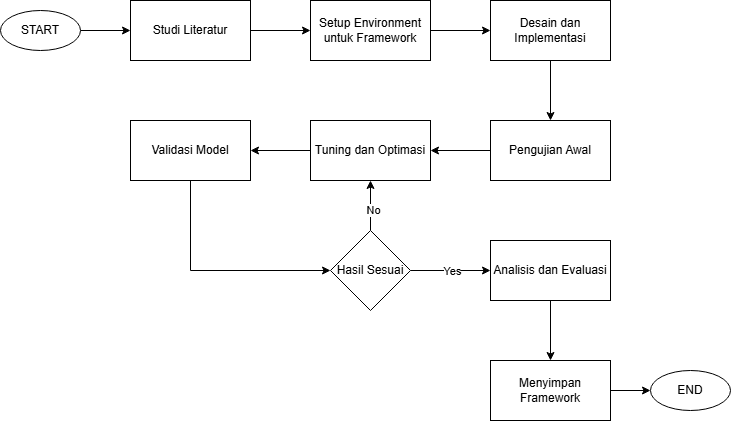
\includegraphics[width=0.95\textwidth]
		{assets/pics/Alur Penelitian.png}
	\caption{Diagram Alur Penelitian}
	\label{fig:testGambar}
\end{figure}

Alur penelitian ini dimulai dengan studi literatur, di mana peneliti mengumpulkan referensi terkait konsep Command and Control (C2), PowerShell, keystroke injection, dan perangkat Digispark. Setelah itu, dilakukan setup environment untuk framework, termasuk pengaturan server C2, perangkat korban, dan perangkat Digispark sebagai media keystroke injection.


Langkah berikutnya adalah desain dan implementasi, yang mencakup perancangan komponen framework serta pengintegrasian modul PowerShell dan Digispark. Setelah framework selesai dikembangkan, dilakukan pengujian awal untuk mengevaluasi performanya dalam skenario simulasi serangan. Jika hasil pengujian tidak sesuai dengan ekspektasi, penelitian dilanjutkan dengan tuning dan optimasi, di mana parameter framework diperbaiki dan diuji ulang hingga mendapatkan hasil yang diinginkan.


Setelah hasil sesuai, framework dievaluasi secara menyeluruh dalam tahap analisis dan evaluasi, untuk memastikan efektivitas dan fungsionalitasnya. Penelitian diakhiri dengan menyimpan framework dalam bentuk final yang siap untuk digunakan dan didokumentasikan.

%-----------------------------------------------------------------------------%
\section{Setup Environment}
%-----------------------------------------------------------------------------%
Dengan tujuan simulasi serangan siber yang realistis, penulis menggunakan perangkat keras berikut:
\begin{itemize}
    \item CPU   : 13th Gen Intel(R) Core(TM) i5-13500H   2.60 GHz
    \item RAM   : 16.0 GB (15.7 GB usable)
    \item Digispark Rev.3

\end{itemize}

Penulis menggunakan perangkat lunak sebagai berikut:
\begin{itemize}
    \item OS    : Windows 11 (version 22631.4602)
    \item Arduino IDE
    \item Duckuino
    \item Amazone AWS

\end{itemize}


%-----------------------------------------------------------------------------%
\section{Implementasi Framework}
%-----------------------------------------------------------------------------%
Implementasi framework dilakukan dengan beberapa tahapan penting yang saling berkaitan. Tahap pertama adalah pemrograman perangkat Digispark menggunakan Arduino IDE. Dalam proses ini, library DigiKeyboard.h dimanfaatkan untuk memungkinkan Digispark mensimulasikan input keyboard secara otomatis. Script yang diprogram pada Digispark berisi instruksi untuk menyisipkan payload PowerShell ke dalam perangkat target. Payload ini dirancang untuk dapat dieksekusi secara otomatis begitu Digispark tersambung ke perangkat target, sehingga pengguna tidak memerlukan intervensi tambahan.


Tahap kedua adalah pengembangan script PowerShell sebagai bagian dari agen untuk server Command and Control (C2). Script ini dirancang untuk menjalankan fungsi-fungsi penting, seperti mengumpulkan data dari perangkat target, mengirimkan data tersebut ke server C2 yang telah dikonfigurasi di Amazon AWS, serta mengeksekusi perintah yang dikirimkan dari server. Dalam pengembangannya, dilakukan berbagai penyesuaian untuk memastikan kompatibilitas script dengan sistem operasi Windows 11, yang menjadi platform target penelitian ini.


Tahap terakhir adalah integrasi seluruh komponen framework. Dalam tahap ini, Digispark, script payload PowerShell, dan server C2 disatukan dalam sebuah alur kerja yang terkoordinasi. Proses integrasi ini bertujuan untuk memastikan bahwa setiap komponen dapat saling berkomunikasi secara efisien dan mendukung simulasi serangan siber yang telah dirancang. Hasil dari implementasi ini diharapkan dapat menghasilkan framework yang tidak hanya fungsional, tetapi juga fleksibel dalam mensimulasikan berbagai skenario serangan.

%-----------------------------------------------------------------------------%
\section{Pengujian Awal}
Setelah implementasi framework selesai, pengujian awal dilakukan untuk memastikan bahwa setiap komponen bekerja sesuai dengan desain yang direncanakan. Pada tahap ini, simulasi serangan dimulai dengan menggunakan Digispark untuk menyisipkan payload PowerShell ke perangkat target. Setelah payload dieksekusi, perangkat target diharapkan dapat terhubung ke server C2 melalui koneksi yang telah dikonfigurasi.


Hasil dari pengujian awal menunjukkan adanya kendala pada proses komunikasi antara perangkat target dan server C2. Script payload yang dijalankan pada perangkat target tidak berhasil mengirimkan data ke server C2 sebagaimana yang diharapkan. Masalah ini dapat disebabkan oleh beberapa faktor, seperti kesalahan dalam konfigurasi server, ketidaksesuaian format data, atau adanya pembatasan sistem pada perangkat target.


Kendala ini memberikan indikasi bahwa framework memerlukan penyesuaian lebih lanjut untuk memastikan keberhasilan komunikasi antara perangkat target dan server C2. Hasil pengujian awal ini menjadi dasar untuk melakukan tuning dan optimasi pada tahap berikutnya, dengan fokus pada perbaikan script payload, pengaturan ulang server C2, dan peningkatan mekanisme injeksi keystroke pada Digispark.
%-----------------------------------------------------------------------------%

%-----------------------------------------------------------------------------%
\section{Tuning dan Optimasi}
Setelah menemukan kendala pada pengujian awal, proses tuning dan optimasi dilakukan untuk meningkatkan performa framework yang telah dikembangkan. Langkah pertama adalah meninjau kembali script payload PowerShell yang digunakan untuk memastikan bahwa perintah-perintah yang dieksekusi sesuai dengan kebutuhan. Penyesuaian dilakukan pada struktur script, termasuk mekanisme pengiriman data ke server C2. Dalam hal ini, penambahan logging pada script PowerShell membantu dalam mengidentifikasi titik-titik kegagalan selama proses komunikasi berlangsung.


Langkah berikutnya adalah memperbaiki konfigurasi server C2 yang dihosting di Amazon AWS. Proses ini melibatkan pengaturan ulang firewall dan port yang digunakan untuk komunikasi dengan perangkat target. Selain itu, dilakukan verifikasi terhadap parameter protokol yang digunakan, seperti protokol HTTP atau HTTPS, untuk memastikan bahwa koneksi dapat diterima dan diproses oleh server C2 tanpa hambatan.


Perangkat Digispark juga mendapat perhatian dalam proses optimasi ini. Script yang diunggah ke perangkat diperbarui untuk memperbaiki timing eksekusi keystroke, memastikan bahwa payload berhasil dimasukkan ke perangkat target tanpa terdeteksi oleh mekanisme keamanan sistem operasi. Percobaan berulang dilakukan untuk menyempurnakan urutan perintah dan waktu jeda antar-eksekusi agar proses injeksi dapat berjalan lebih cepat dan akurat.


Tahapan tuning dan optimasi ini dilanjutkan dengan simulasi serangan menggunakan framework yang telah diperbarui. Setiap perubahan dievaluasi berdasarkan keberhasilan komunikasi antara perangkat target dan server C2, serta efisiensi injeksi payload oleh Digispark. Hasil dari tahapan ini menunjukkan perbaikan signifikan dalam performa framework, di mana koneksi ke server C2 berhasil dijalin, dan payload dapat dieksekusi dengan baik di perangkat target. Proses tuning dan optimasi ini menjadi kunci untuk memastikan framework dapat digunakan secara efektif dalam mensimulasikan serangan siber yang realistis.
%-----------------------------------------------------------------------------%